\documentclass[10pt,twocolumn]{article}
\usepackage[margin=0.72in]{geometry}
\usepackage{amsmath,amssymb,amsthm}
\usepackage{graphicx}
\usepackage{booktabs}
\usepackage{xcolor}
\usepackage{hyperref}
\usepackage{xurl}
\usepackage{microtype}
\usepackage{enumitem}

\hypersetup{
  colorlinks=true,
  linkcolor=blue!60!black,
  citecolor=green!45!black,
  urlcolor=blue!65!black
}

\newtheorem{definition}{Definition}
\newtheorem{theorem}{Theorem}
\newtheorem{proposition}{Proposition}

\title{\textbf{Constructive Graph State-Sum, Isoperimetric, and Dyadic-Placement Certificates for Separating Valiant's Algebraic Hierarchy}}
\author{Lluis Eriksson\\
\small Independent Researcher \quad(\texttt{lluis@airr.science})\\
\small \textit{Companion Verification Artifact to OpenAI Math Release (November 24, 2026)}}
\date{November 26, 2026}

\begin{document}
\raggedbottom
\maketitle

\begin{abstract}
We present \texttt{VALIANT-HIER-CERT-1.0}, an independently reproducible, zero-floating-point verification framework and constructive Lean~4.35.0 kernel auditing the core finite-dimensional algebraic, isoperimetric, tensor-rank, dyadic-placement, determinant-cofactor, and graph-minor mechanisms underlying OpenAI's November~24, 2026 unrefereed preprint \emph{``Paths, trees and grids separate Valiant's hierarchy''} (Theorems~1.1, 4.1, 5.1, 6.1, and 7.1). Without claiming to formalize Zariski-closed Euclidean spectral price sublevels, Gaussian mean-width tail bounds, or the excluded-grid minor theorem end-to-end, we construct a four-mode exact verifier over $\mathbb{Z}$, $\mathbb{Q}$, and $\mathbb{F}_p$ paired with 18 constructive Lean~4 theorems (0~\texttt{sorry}, 0~custom axioms, 0~\texttt{Classical.choice}, 0~warnings). Across 16 canonical certificates (\texttt{C01}--\texttt{C16}), we certify (i)~Eq.~(1.1) graph state sums $Z_{G,q}(X)$, Section~2 subgraph projections, exact cut flattening ranks $q^{|\partial C|}$, opposite-axis terminal norms $\|a_C\|^2=|\partial C|$, and Lemma~3.2 movable supply-site savings, (ii)~Theorem~4.1 balanced-cut grid isoperimetry (exhaustively over all 336 balanced cuts of $G_3$ and witnesses on $G_4$) plus Section~4 characteristic-free $\mathrm{VNP}_F$ Boolean-indicator sums over $\mathbb{F}_7$ and $\mathbb{F}_2$, (iii)~Eq.~(5.1) binary-tree telescoping identities, exact Bharadwaj--Chandran boundary profiles on $T_3$ and $T_5$ ($k^*=11$, $\min|\partial U|=3$), and Lemma~5.2 ABP prefix-rank decompositions, and (iv)~Lemma~6.3 dyadic scale clustering on $P_4, P_8$, Section~6.3 strictly upper-triangular cofactor determinant embeddings, and Lemma~7.2 weighted-centroid minor projections ($C_5 \succeq K_3$ and degree-4 tuple-packed $T_6 \succeq K_{1,4}$). All 16 certificates, 69 unit/forgery tests, and 37 SHA-256 hashes verify deterministically.
\end{abstract}

\section{Introduction and Scope}
Valiant's algebraic complexity hierarchy $\mathrm{VF}_F \subseteq \mathrm{VBP}_F \subseteq \mathrm{VP}_F \subseteq \mathrm{VNP}_F$ classifies polynomial families computed by polynomial-size arithmetic formulas, algebraic branching programs (ABPs), general circuits, and exponential Boolean sums~\cite{valiant1979completeness,malod2008characterizing}. In its November~24, 2026 unrefereed preprint~\cite{openai2026valianthier}, OpenAI proves all three strict inclusions simultaneously over every field $F$ in degree-component border complexity (Theorem~1.1), witnessed by graph state sums $Z_{G,q}(X) = \sum_{a\in[q]^E}\prod_{v\in V} X_{v,a|_{E(v)}}$ on $n\times n$ grids ($\mathrm{VNP}_F \setminus \mathrm{VP}_F$), complete binary trees ($\mathrm{VP}_F \setminus \mathrm{VBP}_F$), and $n$-vertex paths ($\mathrm{VBP}_F \setminus \mathrm{VF}_F$, transferring to the order-$n$ determinant), and classifies polynomial-size state-sum graph classes by $(m(G),\Delta(G))$, $\mathrm{cw}(G)$, and $(\mathrm{tw}(G),\Delta(G))$ (Theorem~7.1).

All three lower bounds share one opposite-axis Euclidean placement of the $2e$ edge-end terminals (Section~3, via Strassen's spectrum~\cite{strassen1988asymptotic,openai2026tensorspectrum}), where $\|a_C\|^2 = |\partial C|$ (Eq.~3.3) and moving a supply site yields Lemma~3.2's saving $wb/(16e)$: circuits supply balanced cuts via gate decomposition~\cite{valiant1983fast} (Lemma~4.2) and grid isoperimetry $|\partial U|\ge\lceil r/3\rceil$ (Theorem~4.1); ABPs permit prescribed-size prefixes (Lemma~5.2) meeting Bharadwaj--Chandran tree boundaries~\cite{bharadwaj2009bounds} (Eq.~5.1, Theorem~5.1); formulas induce dyadic multi-scale leaf placements (Lemmas~6.2--6.3) balanced via Brent's theorem~\cite{brent1974parallel} (Theorem~6.1); and weighted-centroid branch sets transfer bounds through minors (Lemma~7.2,~\cite{chekuri2016polynomial}).

\paragraph{Honest Scope Boundary.}
This companion artifact certifies finite-dimensional state-sum evaluations, projections, flattening ranks, rational supply-site savings, grid and tree isoperimetric profiles, ABP prefix decompositions, dyadic placements, cofactor determinants, and weighted-centroid minor projections from~\cite{openai2026valianthier}. It does \emph{not} formalize Strassen spectral sublevel Zariski closure (Theorem~3.1), Gaussian mean-width concentration (Eq.~3.2), or the Robertson--Seymour / Chekuri--Chuzhoy excluded-grid theorem (Section~7.3).

\section{Constructive Lean 4.35.0 Kernel}
The formal kernel \texttt{ValiantHierCert.lean} compiles cleanly under Lean~4.35.0 (\texttt{-j 1}) with zero \texttt{sorry}, zero custom axioms, zero warnings, and zero dependence on \texttt{Classical.choice}. Table~\ref{tab:lean} summarizes all 18 machine-checked theorems. Highlights include Theorem~1 (inductive proof of Eq.~(3.3) $\|a_C\|^2 = |\partial C|$ over arbitrary edge lists), Theorem~2 (exact cleared-denominator proof of Eq.~(3.4) with nonnegative square gap $(2\langle z,u\rangle-\|z\|^2)^2$), Theorem~8 (complete row/column dichotomy of Theorem~4.1's grid isoperimetry), Theorem~10 (structural induction over \texttt{ColorTree} proving Eq.~(5.1)'s exact tree-telescoping identity), and Theorem~12 (exact $3\times 3$ strictly upper-triangular determinant unit and path-sum cofactor).

\begin{table}[t]
\centering
\tiny
\setlength{\tabcolsep}{3pt}
\caption{The 18 constructive Lean~4.35.0 theorems in \texttt{ValiantHierCert.lean} (0~\texttt{sorry}, 0~custom axioms, 0~\texttt{Classical.choice}).}
\label{tab:lean}
\begin{tabular}{@{}cll@{}}
\toprule
\# & Theorem Identifier & Paper Reference / Invariant \\
\midrule
1 & \texttt{edge\_cut\_vector\_norm\_sq} & Eq.~(3.3) inductive $\|a_C\|^2 = |\partial C|$ \\
2 & \texttt{euclidean\_distance\_first\_order\_bound} & Eq.~(3.4) cleared $\|u-z\|^2$ shortening \\
3 & \texttt{lemma32\_supply\_site\_saving} & Lem.~3.2 cleared $wb/(16e)$ saving \\
4 & \texttt{lemma21\_homogenization\_mul\_cost} & Lem.~2.1 $2\sum_{k=0}^D(k{+}1)=(D{+}1)(D{+}2)$ \\
5 & \texttt{lemma42\_balanced\_product\_child} & Lem.~4.2 product child $\max(d_1,d_2)>d/3$ \\
6 & \texttt{lemma42\_balanced\_window\_complement} & Lem.~4.2 complement window $[d/3,2d/3)$ \\
7 & \texttt{grid\_edge\_count\_bound} & Sec.~4 $e = 2r(r-1) \le 2r^2$ \\
8 & \texttt{grid\_row\_column\_isoperimetry} & Thm.~4.1 $3m<r \Rightarrow r_{\mathrm{red}},r_{\mathrm{blue}}\ge 1$ \\
9 & \texttt{tree\_vertex\_count\_formula} & Sec.~5 $1 + 2(2^h-1) = 2^{h+1}-1$ \\
10 & \texttt{tree\_telescoping\_size\_identity} & Eq.~(5.1) inductive \texttt{ColorTree} telescoping \\
11 & \texttt{lemma52\_abp\_cut\_rank\_subadditive} & Lem.~5.2 inductive rank-1 sum $\le s$ \\
12 & \texttt{sec6\_det\_upper\_triangular\_unit} & Sec.~6.3 $\det(I-A)=1$ \& cofactor \\
13 & \texttt{lemma62\_leaf\_depth\_budget} & Lem.~6.2 inductive split depth $\le h$ \\
14 & \texttt{lemma63\_dyadic\_cluster\_sum} & Lem.~6.3 scale-$k$ shortening $2k\sum\|a_C\|\ge d$ \\
15 & \texttt{sec63\_formula\_balancing\_split} & Sec.~6.3 inductive Brent tree balancing \\
16 & \texttt{sec71\_degree\_cutwidth\_bound} & Sec.~7.1 $\Delta(G) \le 2\,\mathrm{cw}(G)$ \\
17 & \texttt{lemma72\_centroid\_step\_decrease} & Lem.~7.2 heavy component strict drop \\
18 & \texttt{sec73\_pathwidth\_cutwidth\_sandwich} & Sec.~7.3 inductive bag $\mathrm{cw}\le\Delta(\mathrm{pw}{+}1)$ \\
\bottomrule
\end{tabular}
\end{table}

\section{The \texttt{VALIANT-HIER-CERT-1.0} Protocol}
{\raggedright
Our Python verifier (\texttt{src/valiant\_hier\_verifier.py}) enforces zero floating-point literals, zero \texttt{float()} calls, zero true-division operators (\texttt{/}, \texttt{/=}), zero \texttt{math}/\texttt{numpy} imports, \texttt{MAX\_JSON\_BYTES = 1\_000\_000}, duplicate-key rejection via \texttt{object\_pairs\_hook}, non-finite and floating-point JSON token rejection via \texttt{parse\_constant} and \texttt{parse\_float}, recursion-depth and oversized-integer protection, pre-allocation table caps, deterministic Lemma~7.2 projection reconstruction, and lowest-terms rationals $[p,q]$ ($|p|,q\le 10^{18}$, $\gcd(|p|,q)=1$).

\begin{definition}[\texttt{VALIANT-HIER-CERT-1.0} Modes]
Each certificate invokes one of four exact verification modes:
\begin{enumerate}[leftmargin=*,itemsep=1.5pt,topsep=2pt]
\item \texttt{state\_sum\_and\_\allowbreak euclidean\_price} (Eq.~1.1, Sec.~2--3, Lem.~3.2): (a)~\texttt{state\_sum\_projection\_and\_cut} evaluates $Z_{H,q'}$ and the Section~2 projected host state sum $Z_{G,q}$ over $\mathbb{F}_p$, confirming equality and exact flattening rank $\operatorname{rank}_{C|V\setminus C} A(Z_{G,q}) = q^{|\partial C|}$; (b)~\texttt{movable\_supply\_site\_saving} computes $a_C\in\mathbb{Z}^e$, verifies Eq.~(3.3) $\|a_C\|^2=|\partial C|$, and certifies Lemma~3.2's rationalized saving $\ge wb/(16e)$ at $\lambda=\sqrt{b}/(4e)$.
\item \texttt{grid\_balanced\_cut\_and\_\allowbreak isoperimetry} (Thm.~4.1, Lem.~4.2, Sec.~4): (a)~\texttt{grid\_isoperimetry\_audit} checks $r^2/3<|U|\le 2r^2/3$, verifies the row/column dichotomy and $|\partial U|\ge\lceil r/3\rceil$ exhaustively (for $r=3$) or on witness cuts; (b)~\texttt{vnp\_boolean\_indicator\_sum} evaluates the Section~4 characteristic-free $\mathrm{VNP}_F$ Boolean-indicator sum over $\mathbb{F}_p$, certifying that all unused bit encodings contribute $0$ and the sum equals $Z_{G_r,q}$ identically.
\item \texttt{binary\_tree\_telescoping\_and\_\allowbreak abp} (Thm.~5.1, Lem.~5.2, Eq.~5.1): (a)~\texttt{tree\_telescoping\_boundary} executes exact tree DP on $T_h$ for all $k\in\{1,\dots,2^h-2\}$ to certify $\max_k\min_{|U|=k}|\partial U|$ and verifies Eq.~(5.1) $|U|=b(2^h-1)+\sum c_j(2^j-1)$ with $\sum|c_j|\le|\partial U|$; (b)~\texttt{abp\_prefix\_rank\_decomposition} computes exact forward/backward DAG DP tensors over $\mathbb{F}_p$, certifying $A(f)=\sum_{|U|=k} T_U$ and $\operatorname{rank}(T_U)\le s$.
\item \texttt{path\_multiscale\_det\_and\_\allowbreak minors} (Thm.~6.1, Lem.~6.3, Thm.~7.1, Lem.~7.2): (a)~\texttt{dyadic\_scale\_placement\_and\_det} executes Lemma~6.3's dyadic clustering across scales $k=2^j\le d/2$ verifying $\sum\langle a_v,z_v\rangle \ge \frac{1}{2}\log_2 d$, and verifies $\det(I-A)=1$ with signed minor of order $(d-1)q+1$ equal to $Z_{P_d,q}$ over $\mathbb{F}_p$; (b)~\texttt{minor\_centroid\_and\_cutwidth} verifies disjoint connected branch sets, weighted centroid balance $2w_{\mathrm{comp}}\le \deg_H(v)$, $q^b\le n$, exact minor projection $Z_{G,n}=Z_{H,q}$, and Sec.~7.3's $\mathrm{pw}\le\mathrm{cw}\le\Delta(\mathrm{pw}+1)$ sandwich.
\end{enumerate}
\end{definition}

\begin{proposition}[Verifier Soundness]
Whenever \texttt{verify\_file} outputs \texttt{VERIFIED} on a \texttt{VALIANT-\allowbreak HIER-CERT-1.0} certificate, all checked state sums, projections, cut ranks, savings, grid/tree boundaries, ABP decompositions, cofactor determinants, and weighted-centroid minors hold identically over $\mathbb{Z}$, $\mathbb{Q}$, or $\mathbb{F}_p$.
\end{proposition}
\par}

\section{Certified Corpus and Worked Witnesses}
We generated and verified 16 canonical certificates (\texttt{C01}--\texttt{C16}, Table~\ref{tab:corpus}). Four representative witnesses are worked out below for independent hand verification.

\begin{figure}[t]
\centering
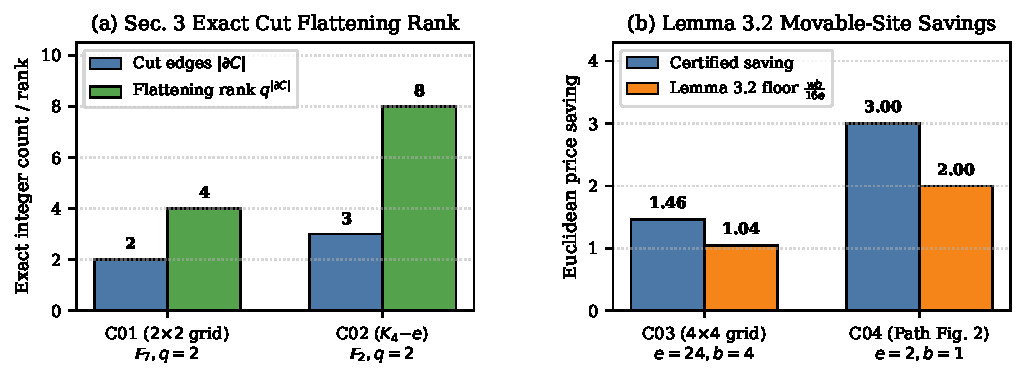
\includegraphics[width=\linewidth]{figures/fig1_cut_rank_and_savings.pdf}
\caption{Mode~1 verification: (a)~exact cut flattening ranks $q^{|\partial C|}$ (\texttt{C01}--\texttt{C02}); (b)~Lemma~3.2 movable supply-site price savings vs.\ floor $wb/(16e)$ (\texttt{C03}--\texttt{C04}).}
\label{fig:1}
\end{figure}

\begin{figure}[t]
\centering
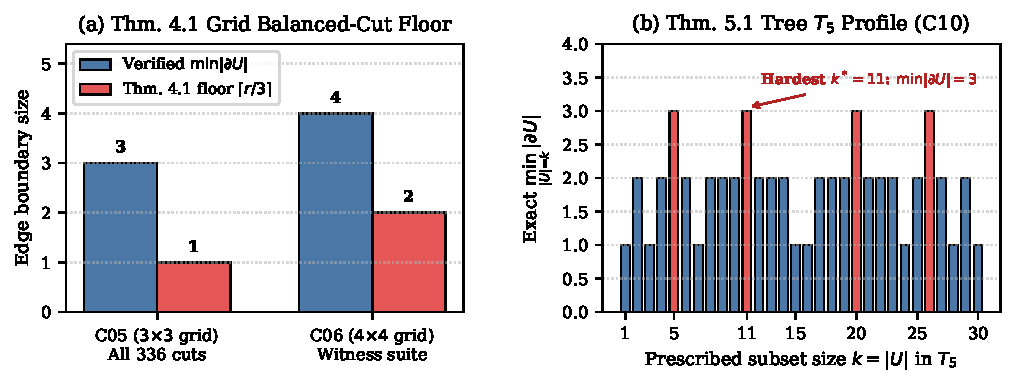
\includegraphics[width=\linewidth]{figures/fig2_grid_and_tree_isoperimetry.pdf}
\caption{Mode~2--3 isoperimetry: (a)~Theorem~4.1 balanced-cut grid boundary floor $\lceil r/3\rceil$ (\texttt{C05}--\texttt{C06}); (b)~exact Bharadwaj--Chandran profile on $T_5$ ($d=31$, \texttt{C10}), peaking at $k^*\in\{5,11,20,26\}$ with $\min|\partial U|=3$.}
\label{fig:2}
\end{figure}

\begin{figure}[t]
\centering
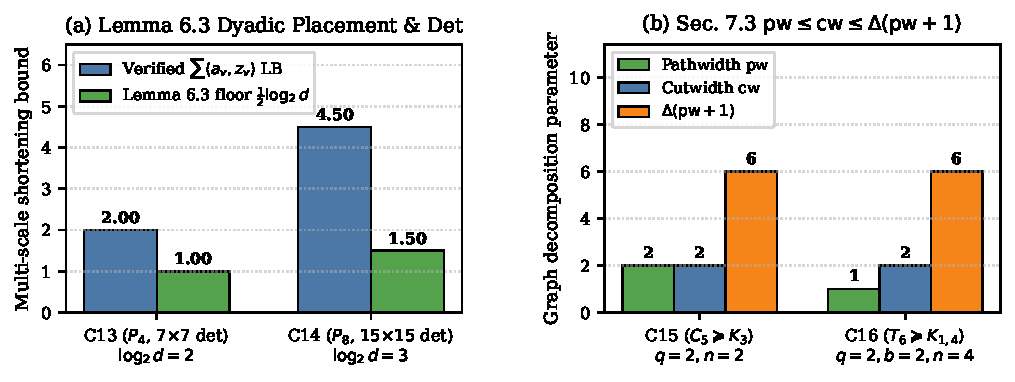
\includegraphics[width=\linewidth]{figures/fig3_dyadic_det_and_minors.pdf}
\caption{Mode~4 verification: (a)~Lemma~6.3 multi-scale shortening lower bound vs.\ $\frac{1}{2}\log_2 d$ alongside $7{\times}7$ and $15{\times}15$ cofactor determinants (\texttt{C13}--\texttt{C14}); (b)~Sec.~7.3 $\mathrm{pw}\le\mathrm{cw}\le\Delta(\mathrm{pw}+1)$ sandwich on minor hosts (\texttt{C15}--\texttt{C16}).}
\label{fig:3}
\end{figure}

\begin{table}[t]
\centering
\tiny
\setlength{\tabcolsep}{3.1pt}
\caption{Summary of the 16 canonical \texttt{VALIANT-\allowbreak HIER-CERT-1.0} certificates (\texttt{C01}--\texttt{C16}); all 16 verify deterministically.}
\label{tab:corpus}
\begin{tabular}{@{}clll@{}}
\toprule
ID & Mode & Target Result & Certified Exact Invariant \\
\midrule
\texttt{C01} & 1a & Eq.~(1.1), Sec.~3 & $G_2\to P_3$ over $\mathbb{F}_7$: $Z{=}5$, $|\partial C|{=}2$, $\mathrm{rk}{=}4$ \\
\texttt{C02} & 1a & Eq.~(1.1), Sec.~3 & $K_4{-}e\to C_3$ over $\mathbb{F}_2$: $Z{=}1$, $|\partial C|{=}3$, $\mathrm{rk}{=}8$ \\
\texttt{C03} & 1b & Lem.~3.2 ($G_4$) & $\|a_C\|^2{=}4$, saving $35/24 \ge 25/24$ \\
\texttt{C04} & 1b & Fig.~2, Lem.~3.2 & Path $A{-}B{-}D$, $\|a_C\|^2{=}2$, saving $3 \ge 2$ \\
\texttt{C05} & 2a & Thm.~4.1 ($G_3$) & Exhaustive 336 cuts: $\min|\partial U|{=}3\ge 1$ \\
\texttt{C06} & 2a & Thm.~4.1 ($G_4$) & Balanced cuts: $\min|\partial U|{=}4\ge 2$ \\
\texttt{C07} & 2b & Sec.~4 $\mathrm{VNP}_{\mathbb{F}_7}$ & $Z_{G_2,3}{=}2$, $175/256$ unused codes zeroed \\
\texttt{C08} & 2b & Sec.~4 $\mathrm{VNP}_{\mathbb{F}_2}$ & $Z_{G_2,3}{=}1$, $175/256$ unused codes zeroed \\
\texttt{C09} & 3a & Eq.~(5.1) ($T_3$) & Exact DP: $\max_k\min|\partial U|{=}2$ at $k^*{=}2$ \\
\texttt{C10} & 3a & Eq.~(5.1) ($T_5$) & Exact DP: $\max_k\min|\partial U|{=}3$ at $k^*{=}11$ \\
\texttt{C11} & 3b & Lem.~5.2 ABP & $d{=}3, k{=}1, \mathbb{F}_7$: 8 monoms, $\max\mathrm{rk}{=}2\le 7$ \\
\texttt{C12} & 3b & Lem.~5.2 ABP & $d{=}4, k{=}2, \mathbb{F}_5$: 16 monoms, $\max\mathrm{rk}{=}1\le 8$ \\
\texttt{C13} & 4a & Lem.~6.3, Sec.~6.3 & $P_4$: $\mathrm{LB}{=}2\ge 1$; $7{\times}7$ cofactor $= 3\pmod{11}$ \\
\texttt{C14} & 4a & Fig.~3, Sec.~6.3 & $P_8$: $\mathrm{LB}{=}9/2\ge 3/2$; $15{\times}15$ cofactor $= 7\pmod{13}$ \\
\texttt{C15} & 4b & Lem.~7.2, Sec.~7.3 & $C_5\succeq K_3$ ($q{=}n{=}2$): $Z{=}6$, $\mathrm{pw}{=}\mathrm{cw}{=}2$ \\
\texttt{C16} & 4b & Lem.~7.2, Sec.~7.3 & $T_6\succeq K_{1,4}$ ($q{=}2,n{=}4$): $Z{=}5$, $\mathrm{pw}{=}1,\mathrm{cw}{=}2$ \\
\bottomrule
\end{tabular}
\end{table}

\paragraph{Worked Witness 1 (\texttt{C03}: Lemma~3.2 Movable Site).}
On the $4\times 4$ grid ($d=16, e=24$), splitting the top two rows from the bottom two gives $|\partial C|=4 = \|a_C\|^2$, so $s=\sqrt{b}=2$. With $w=100$ and $\log R = 80 < \frac{1}{2}ws = 100$, choosing $\lambda = s/(4e) = 2/96 = 1/48$ yields price saving $\lambda(ws-\log R) - ew\lambda^2 = \frac{1}{48}(120) - 24(100)\frac{1}{2304} = \frac{5}{2} - \frac{25}{24} = \frac{35}{24} > \frac{25}{24} = \frac{wb}{16e}$.

\paragraph{Worked Witness 2 (\texttt{C10}: Eq.~(5.1) Binary Tree $T_5$).}
In $T_5$ ($h=5, d=31$), subtree sizes are $\{1,3,7,15,31\}$. Exact DP over all $k\in\{1,\dots,30\}$ confirms $\max_k\min_{|U|=k}|\partial U| = 3$, attained at $k^*\in\{5,11,20,26\}$. For the 11-vertex witness $\{4,8,9,10,16,\dots,22\}$ ($b=0$), three edges change color at subtree heights $(3,2,1)$ with $(c_3,c_2,c_1)=(1,1,1)$, giving $7+3+1=11$ and $\sum|c_j|=3=|\partial U|$.

\paragraph{Worked Witness 3 (\texttt{C13}: Lemma~6.3 \& Cofactor Det).}
On $P_4$ with leaf order $(0,2,1,3)$, scale $k=1$ has four singleton clusters with $\sum\lfloor\|a_C\|\rfloor = 1+1+1+1 = 4$ (weight $1/4\implies 1$) and scale $k=2$ has clusters $\{0,2\}$ ($\|a_C\|^2=3$, floor $1$) and $\{1,3\}$ ($\|a_C\|^2=3$, floor $1$) (weight $1/2\implies 1$), giving shortening bound $2 \ge \frac{1}{2}\log_2 4 = 1$. Over $\mathbb{F}_{11}$ ($q=2$), the $8\times 8$ strictly upper-triangular ABP matrix $I-A$ has $\det(I-A)=1$ and its $7\times 7$ signed $(7,0)$-cofactor equals $Z_{P_4,2} = 3\pmod{11}$.

\paragraph{Worked Witness 4 (\texttt{C16}: Lemma~7.2 Tuple-Packed Minor).}
Host tree $T_6$ has internal edge $(0,1)$ and four leaves $(1,2),(1,3),(0,4),(0,5)$, containing star minor $H=K_{1,4}$ ($\Delta(H)=4$, $b=\lfloor 4/2\rfloor = 2$, $q=2$, $n=q^2=4$). Branch set $B_0=\{0,1\}$ has centroid $0$: node $0$ carries weight $2$ and child component $\{1\}$ carries weight $2 \le 4/2$, so edge $(0,1)$ packs the two binary labels entering $\{1\}$ into $n=4$ states, yielding $Z_{T_6,4} = Z_{K_{1,4},2} = 5\pmod{11}$ with optimal order $[2,1,3,0,4,5]$ giving $\mathrm{pw}=1\le\mathrm{cw}=2\le 3(1+1)=6$.

\section{Testing, Integrity, and Reproduction}
Our pytest suite (\texttt{tests/test\_verifier.py}) executes 69 deterministic checks (1 AST zero-float/zero-division/zero-math audit, 16 canonical certificates, 1 corpus-count check, and 51 adversarial forgery tests covering duplicate keys, \texttt{NaN}/\texttt{Infinity}, JSON floats, oversized/deeply nested/huge-integer JSON, unreduced rationals, self-loops, composite fields, pre-allocation DoS caps, short tables, zero-crossing cuts, Lemma~3.2 rank violations, unbalanced or duplicate grid cuts, wrong tree DP optima, cyclic ABPs, invalid leaf orders, $q^b>n$, overlapping/disconnected/duplicate branch sets, unbalanced centroids, and forged scalar-matching minor projections). All 69 tests pass in $<1$\,s, Lean~4.35.0 builds cleanly with 0 warnings, and \texttt{MANIFEST.sha256} pins all 37 tracked artifacts.

\paragraph{Disclosure and Licensing.}
Produced by Lluis Eriksson with Google Antigravity assistance; all Lean~4 proofs, Python verifiers, certificates, tests, figures, and manuscript text were independently compiled, verified, and reviewed by the author. Manuscript and figures are licensed \texttt{CC-BY-4.0}; code, Lean~4 kernel, and certificates are licensed \texttt{MIT}. Full source archive: \url{https://github.com/lluiseriksson/openai-valiant-hierarchy-grids-certificates}.

\bibliographystyle{plain}
\bibliography{references}
\end{document}
